\documentclass[../main]{subfiles}

\questiontrue
\solutiontrue

\begin{document}
    \ifquestion
    
	
\section{"Relative" Luminosity}

In this problem, we aim to find an expression for the distribution of luminous power of a spherical wavefront emitted from a source in a reference frame $S'$, which emits light isotropically with total power $L$ and moves with velocity $v = \beta c$.

Before that, however, we will review some of the principles governing special relativity, so that we can proceed with the calculations.

\parte{A}{Lorentz Transformations}

A transformation is nothing more than the relation between the coordinates of two reference frames, $S$ and $S'$. In the following derivations, consider $S$ as the stationary frame of an external observer and $S'$ as the frame moving with velocity $v$ along the $x$-axis relative to $S$.

Imagine that at the moment the origins of the two frames coincide, a light ray is emitted from the origin.  

\ut{A.1} Show that:

$$x^2 + y^2 + z^2 - (ct)^2 = x'^2 + y'^2 + z'^2 - (ct')^2$$

where $x', y', z' \text{ and } t'$ are the coordinates in $S'$.

\ut{A.2} Argue, by contradiction, the necessity that $y = y'$ and $z = z'$ (note that this is not required for $x$ or $t$).

\ut{A.3} Note that in this way, it follows that $x^2 - (ct)^2 = x'^2 - (ct')^2$. Observe that this description is very similar to the squared modulus of a two-dimensional vector ($|\vec{v}|^2 = v_x^2 + v_y^2$), which remains constant after a given transformation. A linear transformation with this property is a rotation. Considering that in the transformation $S \rightarrow S'$, along the appropriate axes, there is a rotation by an angle $\theta$, find the relation $x \rightarrow x'$ and $t \rightarrow t'$.

\ut{A.4} Finally, find the Lorentz transformations, that is, the relation between coordinates in the two reference frames.

\begin{doublespace}

\begin{large}
\textbf{Part B: Headlight Effect}
\end{large}

\end{doublespace}

\ut{B.1} Find the power $dL'$ passing through the area on the sphere (see the figure below) delimited by an angular interval $d\theta'$ from the $x'$-axis, as shown in \autoref{fig:NaN}. Express the result in terms of the total power $L$, the angle $\theta'$, and $d\theta'$.

\clearpage

\begin{figure}
    \centering
    \includegraphics[scale=0.6]{images/circ.PNG}
    \caption{Representation of the considered angular interval}
    \label{fig:NaN}
\end{figure}

\ut{B.2} Consider a light beam propagating at an angle $\theta'$ with respect to the $x'$-axis (figure below). In the reference frame $S$, this angle is $\theta$. Find an expression relating $\theta$ and $\theta'$.
	
	    \begin{figure}[htpb]
        \centering
        
\tikzset{every picture/.style={line width=0.75pt}} %set default line width to 0.75pt        

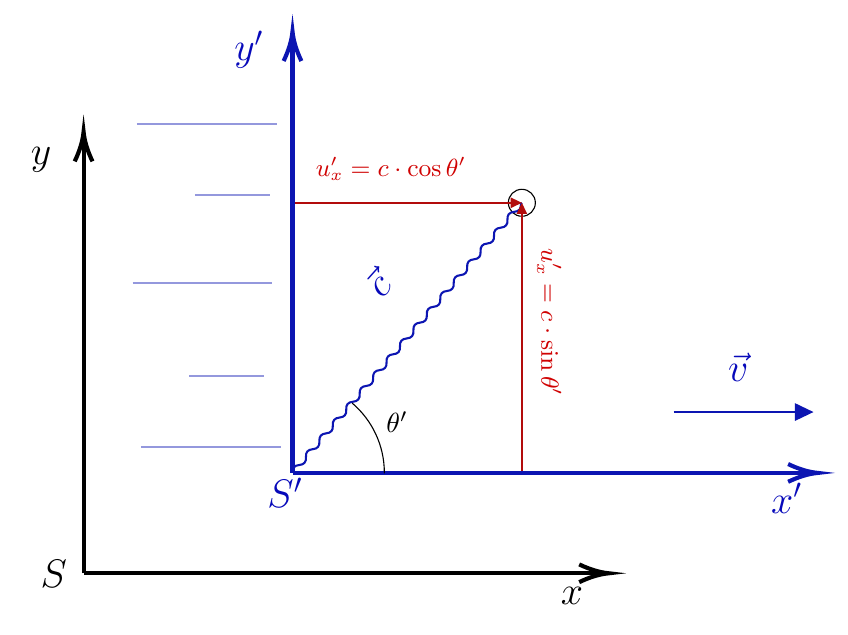
\begin{tikzpicture}[x=0.75pt,y=0.75pt,yscale=-1,xscale=1]
%uncomment if require: \path (0,408); %set diagram left start at 0, and has height of 408

%Straight Lines [id:da035704593072243496] 
\draw [line width=1.5]    (94.67,358.01) -- (94.67,148.34) ;
\draw [shift={(94.67,145.34)}, rotate = 90] [color={rgb, 255:red, 0; green, 0; blue, 0 }  ][line width=1.5]    (14.21,-4.28) .. controls (9.04,-1.82) and (4.3,-0.39) .. (0,0) .. controls (4.3,0.39) and (9.04,1.82) .. (14.21,4.28)   ;
%Straight Lines [id:da6185871938411547] 
\draw [line width=1.5]    (94.67,358.01) -- (344.67,358.01) ;
\draw [shift={(347.67,358.01)}, rotate = 180] [color={rgb, 255:red, 0; green, 0; blue, 0 }  ][line width=1.5]    (14.21,-4.28) .. controls (9.04,-1.82) and (4.3,-0.39) .. (0,0) .. controls (4.3,0.39) and (9.04,1.82) .. (14.21,4.28)   ;
%Straight Lines [id:da699063725695984] 
\draw [color={rgb, 255:red, 12; green, 21; blue, 178 }  ,draw opacity=1 ][line width=1.5]    (195.33,309.66) -- (195.33,99.99) ;
\draw [shift={(195.33,96.99)}, rotate = 90] [color={rgb, 255:red, 12; green, 21; blue, 178 }  ,draw opacity=1 ][line width=1.5]    (14.21,-4.28) .. controls (9.04,-1.82) and (4.3,-0.39) .. (0,0) .. controls (4.3,0.39) and (9.04,1.82) .. (14.21,4.28)   ;
%Straight Lines [id:da10168494105738768] 
\draw [color={rgb, 255:red, 12; green, 21; blue, 178 }  ,draw opacity=1 ][line width=1.5]    (195.33,309.66) -- (445.33,309.66) ;
\draw [shift={(448.33,309.66)}, rotate = 180] [color={rgb, 255:red, 12; green, 21; blue, 178 }  ,draw opacity=1 ][line width=1.5]    (14.21,-4.28) .. controls (9.04,-1.82) and (4.3,-0.39) .. (0,0) .. controls (4.3,0.39) and (9.04,1.82) .. (14.21,4.28)   ;
%Straight Lines [id:da19935241186224828] 
\draw [color={rgb, 255:red, 12; green, 21; blue, 178 }  ,draw opacity=1 ][line width=0.75]    (379,280.33) -- (443.33,280.33) ;
\draw [shift={(446.33,280.33)}, rotate = 180] [fill={rgb, 255:red, 12; green, 21; blue, 178 }  ,fill opacity=1 ][line width=0.08]  [draw opacity=0] (8.93,-4.29) -- (0,0) -- (8.93,4.29) -- cycle    ;
%Shape: Circle [id:dp5740094199155588] 
\draw   (299.33,179.51) .. controls (299.33,175.92) and (302.24,173.01) .. (305.83,173.01) .. controls (309.42,173.01) and (312.33,175.92) .. (312.33,179.51) .. controls (312.33,183.1) and (309.42,186.01) .. (305.83,186.01) .. controls (302.24,186.01) and (299.33,183.1) .. (299.33,179.51) -- cycle ;
%Straight Lines [id:da39046452059581926] 
\draw [color={rgb, 255:red, 12; green, 21; blue, 178 }  ,draw opacity=1 ][line width=0.75]    (195.33,309.66) .. controls (195.14,307.31) and (196.22,306.04) .. (198.57,305.85) .. controls (200.92,305.66) and (202,304.39) .. (201.81,302.04) .. controls (201.62,299.69) and (202.69,298.42) .. (205.04,298.23) .. controls (207.39,298.04) and (208.47,296.77) .. (208.28,294.42) .. controls (208.09,292.07) and (209.16,290.8) .. (211.51,290.6) .. controls (213.86,290.41) and (214.94,289.14) .. (214.75,286.79) .. controls (214.56,284.44) and (215.64,283.17) .. (217.99,282.98) .. controls (220.34,282.79) and (221.41,281.52) .. (221.22,279.17) .. controls (221.03,276.82) and (222.11,275.55) .. (224.46,275.36) .. controls (226.81,275.17) and (227.88,273.9) .. (227.69,271.55) .. controls (227.5,269.2) and (228.58,267.92) .. (230.93,267.73) .. controls (233.28,267.54) and (234.36,266.27) .. (234.17,263.92) .. controls (233.98,261.57) and (235.05,260.3) .. (237.4,260.11) .. controls (239.75,259.92) and (240.83,258.65) .. (240.64,256.3) .. controls (240.45,253.95) and (241.52,252.68) .. (243.87,252.49) .. controls (246.22,252.3) and (247.3,251.03) .. (247.11,248.68) .. controls (246.92,246.33) and (248,245.06) .. (250.35,244.87) .. controls (252.7,244.67) and (253.77,243.4) .. (253.58,241.05) .. controls (253.39,238.7) and (254.47,237.43) .. (256.82,237.24) .. controls (259.17,237.05) and (260.24,235.78) .. (260.05,233.43) .. controls (259.86,231.08) and (260.94,229.81) .. (263.29,229.62) .. controls (265.64,229.43) and (266.72,228.16) .. (266.53,225.81) .. controls (266.34,223.46) and (267.41,222.19) .. (269.76,222) .. controls (272.11,221.81) and (273.19,220.53) .. (273,218.18) .. controls (272.81,215.83) and (273.88,214.56) .. (276.23,214.37) .. controls (278.58,214.18) and (279.66,212.91) .. (279.47,210.56) .. controls (279.28,208.21) and (280.36,206.94) .. (282.71,206.75) .. controls (285.06,206.56) and (286.13,205.29) .. (285.94,202.94) .. controls (285.75,200.59) and (286.83,199.32) .. (289.18,199.13) .. controls (291.53,198.94) and (292.61,197.66) .. (292.42,195.31) .. controls (292.23,192.96) and (293.3,191.69) .. (295.65,191.5) .. controls (298,191.31) and (299.08,190.04) .. (298.89,187.69) .. controls (298.7,185.34) and (299.77,184.07) .. (302.12,183.88) .. controls (304.47,183.69) and (305.55,182.42) .. (305.36,180.07) -- (305.83,179.51) -- (305.83,179.51) ;
%Straight Lines [id:da2956236916778816] 
\draw [color={rgb, 255:red, 12; green, 21; blue, 178 }  ,draw opacity=0.44 ][line width=0.75]    (120.33,141.66) -- (187.67,141.66) ;
%Straight Lines [id:da06275454047861562] 
\draw [color={rgb, 255:red, 12; green, 21; blue, 178 }  ,draw opacity=0.44 ][line width=0.75]    (148.33,175.66) -- (184.33,175.66) ;
%Straight Lines [id:da6151819284038151] 
\draw [color={rgb, 255:red, 12; green, 21; blue, 178 }  ,draw opacity=0.44 ][line width=0.75]    (118.33,218.33) -- (185.67,218.33) ;
%Straight Lines [id:da4492087263895772] 
\draw [color={rgb, 255:red, 12; green, 21; blue, 178 }  ,draw opacity=0.44 ][line width=0.75]    (122.33,296.99) -- (189.67,296.99) ;
%Straight Lines [id:da6632850248594533] 
\draw [color={rgb, 255:red, 12; green, 21; blue, 178 }  ,draw opacity=0.44 ][line width=0.75]    (145.67,262.99) -- (181.67,262.99) ;
%Straight Lines [id:da3436387173601163] 
\draw [color={rgb, 255:red, 178; green, 12; blue, 12 }  ,draw opacity=1 ][line width=0.75]    (196.33,179.51) -- (302.83,179.51) ;
\draw [shift={(305.83,179.51)}, rotate = 180] [fill={rgb, 255:red, 178; green, 12; blue, 12 }  ,fill opacity=1 ][line width=0.08]  [draw opacity=0] (5.36,-2.57) -- (0,0) -- (5.36,2.57) -- cycle    ;
%Straight Lines [id:da6284992247502972] 
\draw [color={rgb, 255:red, 178; green, 12; blue, 12 }  ,draw opacity=1 ][line width=0.75]    (305.83,308.68) -- (305.83,182.51) ;
\draw [shift={(305.83,179.51)}, rotate = 90] [fill={rgb, 255:red, 178; green, 12; blue, 12 }  ,fill opacity=1 ][line width=0.08]  [draw opacity=0] (5.36,-2.57) -- (0,0) -- (5.36,2.57) -- cycle    ;
%Shape: Arc [id:dp25464527059767583] 
\draw  [draw opacity=0] (224.1,276.03) .. controls (233.58,284.15) and (239.58,296.2) .. (239.58,309.66) .. controls (239.58,309.74) and (239.58,309.82) .. (239.58,309.89) -- (195.33,309.66) -- cycle ; \draw   (224.1,276.03) .. controls (233.58,284.15) and (239.58,296.2) .. (239.58,309.66) .. controls (239.58,309.74) and (239.58,309.82) .. (239.58,309.89) ;  

% Text Node
\draw (68,151.41) node [anchor=north west][inner sep=0.75pt]  [font=\Large]  {$y$};
% Text Node
\draw (323.33,363.41) node [anchor=north west][inner sep=0.75pt]  [font=\Large]  {$x$};
% Text Node
\draw (166,95.41) node [anchor=north west][inner sep=0.75pt]  [font=\Large,color={rgb, 255:red, 7; green, 9; blue, 186 }  ,opacity=1 ]  {$y'$};
% Text Node
\draw (424.67,313.41) node [anchor=north west][inner sep=0.75pt]  [font=\Large,color={rgb, 255:red, 7; green, 9; blue, 186 }  ,opacity=1 ]  {$x'$};
% Text Node
\draw (72.67,350.41) node [anchor=north west][inner sep=0.75pt]  [font=\Large]  {$S$};
% Text Node
\draw (182,310.74) node [anchor=north west][inner sep=0.75pt]  [font=\Large,color={rgb, 255:red, 7; green, 9; blue, 186 }  ,opacity=1 ]  {$S'$};
% Text Node
\draw (404,250.74) node [anchor=north west][inner sep=0.75pt]  [font=\Large,color={rgb, 255:red, 7; green, 9; blue, 186 }  ,opacity=1 ]  {$\vec{v}$};
% Text Node
\draw (226.87,217.15) node [anchor=north west][inner sep=0.75pt]  [font=\Large,color={rgb, 255:red, 7; green, 9; blue, 186 }  ,opacity=1 ,rotate=-311.86]  {$\vec{c}$};
% Text Node
\draw (205.33,156.08) node [anchor=north west][inner sep=0.75pt]  [font=\small,color={rgb, 255:red, 208; green, 2; blue, 2 }  ,opacity=1 ]  {$u_{x} '=c\cdot \cos \theta '$};
% Text Node
\draw (326.1,200.51) node [anchor=north west][inner sep=0.75pt]  [font=\small,color={rgb, 255:red, 208; green, 2; blue, 2 }  ,opacity=1 ,rotate=-90]  {$u_{x} '=c\cdot \sin \theta '$};
% Text Node
\draw (239.33,278.74) node [anchor=north west][inner sep=0.75pt]    {$\theta '$};


\end{tikzpicture}

\caption{Headlight effect applied to the change in light propagation angle with the change of reference frame}
\label{fig:relative}
\end{figure}

\ut{B.3} From the previous result, find the value of $d\theta'$ as a function of $d\theta$ and $\theta$.

\begin{doublespace}

\begin{large}
\textbf{Part C: Redshift and Blueshift}
\end{large}

\end{doublespace}

Now we will consider the effects of changes in the frequency of light emitted due to relativistic effects of the source. Note that this change is also related to the energy of photons: $E \propto f$.

	\begin{figure}[htpb]
	    \centering
	    

\tikzset{every picture/.style={line width=0.75pt}} %set default line width to 0.75pt        

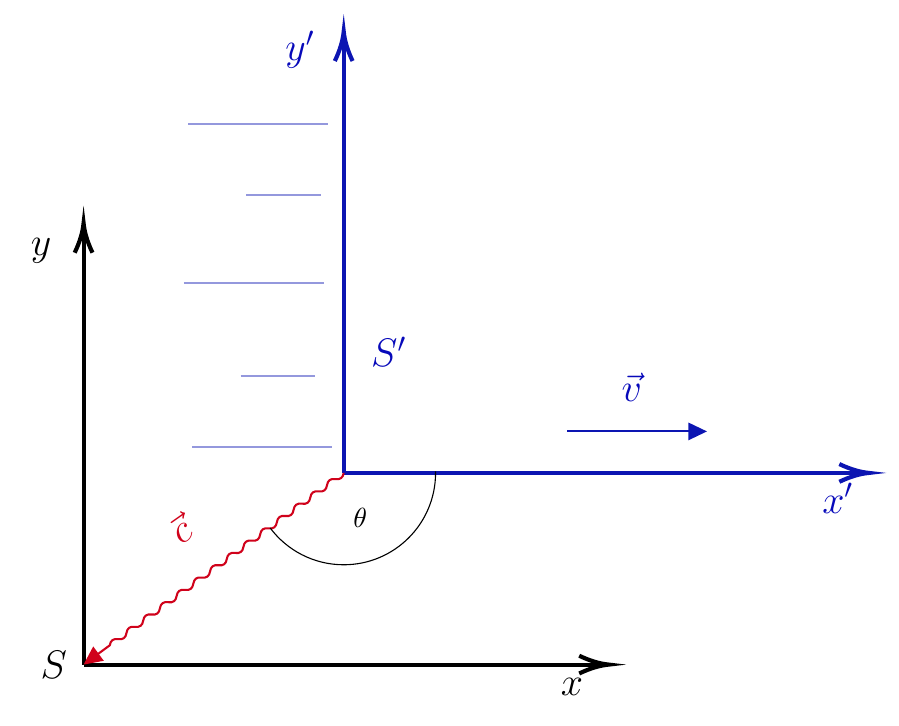
\begin{tikzpicture}[x=0.75pt,y=0.75pt,yscale=-1,xscale=1]
%uncomment if require: \path (0,408); %set diagram left start at 0, and has height of 408

%Straight Lines [id:da035704593072243496] 
\draw [line width=1.5]    (94.67,358.01) -- (94.67,148.34) ;
\draw [shift={(94.67,145.34)}, rotate = 90] [color={rgb, 255:red, 0; green, 0; blue, 0 }  ][line width=1.5]    (14.21,-4.28) .. controls (9.04,-1.82) and (4.3,-0.39) .. (0,0) .. controls (4.3,0.39) and (9.04,1.82) .. (14.21,4.28)   ;
%Straight Lines [id:da6185871938411547] 
\draw [line width=1.5]    (94.67,358.01) -- (344.67,358.01) ;
\draw [shift={(347.67,358.01)}, rotate = 180] [color={rgb, 255:red, 0; green, 0; blue, 0 }  ][line width=1.5]    (14.21,-4.28) .. controls (9.04,-1.82) and (4.3,-0.39) .. (0,0) .. controls (4.3,0.39) and (9.04,1.82) .. (14.21,4.28)   ;
%Straight Lines [id:da699063725695984] 
\draw [color={rgb, 255:red, 12; green, 21; blue, 178 }  ,draw opacity=1 ][line width=1.5]    (220,265.66) -- (220,55.99) ;
\draw [shift={(220,52.99)}, rotate = 90] [color={rgb, 255:red, 12; green, 21; blue, 178 }  ,draw opacity=1 ][line width=1.5]    (14.21,-4.28) .. controls (9.04,-1.82) and (4.3,-0.39) .. (0,0) .. controls (4.3,0.39) and (9.04,1.82) .. (14.21,4.28)   ;
%Straight Lines [id:da10168494105738768] 
\draw [color={rgb, 255:red, 12; green, 21; blue, 178 }  ,draw opacity=1 ][line width=1.5]    (220,265.66) -- (470,265.66) ;
\draw [shift={(473,265.66)}, rotate = 180] [color={rgb, 255:red, 12; green, 21; blue, 178 }  ,draw opacity=1 ][line width=1.5]    (14.21,-4.28) .. controls (9.04,-1.82) and (4.3,-0.39) .. (0,0) .. controls (4.3,0.39) and (9.04,1.82) .. (14.21,4.28)   ;
%Straight Lines [id:da19935241186224828] 
\draw [color={rgb, 255:red, 12; green, 21; blue, 178 }  ,draw opacity=1 ][line width=0.75]    (327.67,245.66) -- (392,245.66) ;
\draw [shift={(395,245.66)}, rotate = 180] [fill={rgb, 255:red, 12; green, 21; blue, 178 }  ,fill opacity=1 ][line width=0.08]  [draw opacity=0] (8.93,-4.29) -- (0,0) -- (8.93,4.29) -- cycle    ;
%Straight Lines [id:da39046452059581926] 
\draw [color={rgb, 255:red, 208; green, 2; blue, 27 }  ,draw opacity=1 ][line width=0.75]    (220,265.66) .. controls (219.65,267.99) and (218.3,268.98) .. (215.97,268.63) .. controls (213.64,268.28) and (212.3,269.26) .. (211.95,271.59) .. controls (211.6,273.92) and (210.25,274.91) .. (207.92,274.56) .. controls (205.59,274.21) and (204.25,275.2) .. (203.9,277.53) .. controls (203.54,279.86) and (202.2,280.84) .. (199.87,280.49) .. controls (197.54,280.14) and (196.2,281.13) .. (195.85,283.46) .. controls (195.49,285.79) and (194.15,286.77) .. (191.82,286.42) .. controls (189.49,286.07) and (188.15,287.06) .. (187.8,289.39) .. controls (187.45,291.72) and (186.1,292.71) .. (183.77,292.36) .. controls (181.44,292.01) and (180.1,292.99) .. (179.75,295.32) .. controls (179.4,297.65) and (178.05,298.64) .. (175.72,298.29) .. controls (173.39,297.94) and (172.05,298.92) .. (171.7,301.25) .. controls (171.35,303.58) and (170,304.57) .. (167.67,304.22) .. controls (165.34,303.87) and (164,304.85) .. (163.65,307.18) .. controls (163.3,309.51) and (161.95,310.5) .. (159.62,310.15) .. controls (157.29,309.8) and (155.95,310.79) .. (155.6,313.12) .. controls (155.24,315.45) and (153.9,316.43) .. (151.57,316.08) .. controls (149.24,315.73) and (147.89,316.72) .. (147.54,319.05) .. controls (147.19,321.38) and (145.85,322.36) .. (143.52,322.01) .. controls (141.19,321.66) and (139.84,322.65) .. (139.49,324.98) .. controls (139.14,327.31) and (137.8,328.3) .. (135.47,327.95) .. controls (133.14,327.6) and (131.8,328.58) .. (131.44,330.91) .. controls (131.09,333.24) and (129.75,334.23) .. (127.42,333.88) .. controls (125.09,333.53) and (123.75,334.51) .. (123.39,336.84) .. controls (123.04,339.17) and (121.7,340.16) .. (119.37,339.81) .. controls (117.04,339.46) and (115.69,340.45) .. (115.34,342.78) .. controls (114.99,345.11) and (113.65,346.09) .. (111.32,345.74) .. controls (108.99,345.39) and (107.64,346.38) .. (107.29,348.71) -- (103.52,351.49) -- (97.08,356.23) ;
\draw [shift={(94.67,358.01)}, rotate = 323.62] [fill={rgb, 255:red, 208; green, 2; blue, 27 }  ,fill opacity=1 ][line width=0.08]  [draw opacity=0] (8.93,-4.29) -- (0,0) -- (8.93,4.29) -- cycle    ;
%Straight Lines [id:da2956236916778816] 
\draw [color={rgb, 255:red, 12; green, 21; blue, 178 }  ,draw opacity=0.44 ][line width=0.75]    (145,97.66) -- (212.33,97.66) ;
%Straight Lines [id:da06275454047861562] 
\draw [color={rgb, 255:red, 12; green, 21; blue, 178 }  ,draw opacity=0.44 ][line width=0.75]    (173,131.66) -- (209,131.66) ;
%Straight Lines [id:da6151819284038151] 
\draw [color={rgb, 255:red, 12; green, 21; blue, 178 }  ,draw opacity=0.44 ][line width=0.75]    (143,174.33) -- (210.33,174.33) ;
%Straight Lines [id:da4492087263895772] 
\draw [color={rgb, 255:red, 12; green, 21; blue, 178 }  ,draw opacity=0.44 ][line width=0.75]    (147,252.99) -- (214.33,252.99) ;
%Straight Lines [id:da6632850248594533] 
\draw [color={rgb, 255:red, 12; green, 21; blue, 178 }  ,draw opacity=0.44 ][line width=0.75]    (170.33,218.99) -- (206.33,218.99) ;
%Shape: Arc [id:dp25464527059767583] 
\draw  [draw opacity=0] (264.24,264.97) .. controls (264.25,265.2) and (264.25,265.43) .. (264.25,265.66) .. controls (264.25,290.1) and (244.44,309.91) .. (220,309.91) .. controls (205.49,309.91) and (192.61,302.93) .. (184.54,292.13) -- (220,265.66) -- cycle ; \draw   (264.24,264.97) .. controls (264.25,265.2) and (264.25,265.43) .. (264.25,265.66) .. controls (264.25,290.1) and (244.44,309.91) .. (220,309.91) .. controls (205.49,309.91) and (192.61,302.93) .. (184.54,292.13) ;  

% Text Node
\draw (68,151.41) node [anchor=north west][inner sep=0.75pt]  [font=\Large]  {$y$};
% Text Node
\draw (323.33,363.41) node [anchor=north west][inner sep=0.75pt]  [font=\Large]  {$x$};
% Text Node
\draw (190.67,51.41) node [anchor=north west][inner sep=0.75pt]  [font=\Large,color={rgb, 255:red, 7; green, 9; blue, 186 }  ,opacity=1 ]  {$y'$};
% Text Node
\draw (449.33,269.41) node [anchor=north west][inner sep=0.75pt]  [font=\Large,color={rgb, 255:red, 7; green, 9; blue, 186 }  ,opacity=1 ]  {$x'$};
% Text Node
\draw (72.67,350.41) node [anchor=north west][inner sep=0.75pt]  [font=\Large]  {$S$};
% Text Node
\draw (232,198.74) node [anchor=north west][inner sep=0.75pt]  [font=\Large,color={rgb, 255:red, 7; green, 9; blue, 186 }  ,opacity=1 ]  {$S'$};
% Text Node
\draw (352.67,216.08) node [anchor=north west][inner sep=0.75pt]  [font=\Large,color={rgb, 255:red, 7; green, 9; blue, 186 }  ,opacity=1 ]  {$\vec{v}$};
% Text Node
\draw (132.11,289.26) node [anchor=north west][inner sep=0.75pt]  [font=\Large,color={rgb, 255:red, 208; green, 2; blue, 27 }  ,opacity=1 ,rotate=-324.81]  {$\vec{c}$};
% Text Node
\draw (223.33,281.41) node [anchor=north west][inner sep=0.75pt]    {$\theta $};


\end{tikzpicture}
	
\caption{Incidence of light from the moving reference frame $S'$ relative to $S$}
\label{fig:refre22}
\end{figure}

\ut{C.1} Considering the received light as a two-dimensional sinusoidal wave (we will analyze only the electric field) with phase $\phi = \vec{k} \cdot \vec{r} - \omega t$, rewrite the phase $\phi$ in terms of the angle $\theta$ and substituting the parameters $\vec{r}$ and $t$ with the parameters of $S'$: $(x',y',t')$.

\textbf{Reminder:} $\vec{r} = \vec{x} + \vec{y}$ and $\vec{k}$ is the angular wave number.

\ut{C.2} Compare the expression from the previous item with the phase $\phi'$ of light emission in the reference frame $S'$ and find the ratio between the received and emitted frequencies.

\begin{doublespace}

\begin{large}
\textbf{Part D: The Grand Unification}
\end{large}

\end{doublespace}

Finally, we aim to find the distribution $dL(\theta)$ of power within the angular interval $d\theta$.

\ut{D.1} Find a relation between $\dfrac{dE}{dt}$ and $\dfrac{dE'}{dt'}$ ($E$ and $E'$ are the energies passing through the angular intervals).

\ut{D.2} Considering that $\dfrac{dE}{dt} = dL(\theta)$, find the distribution function $dL(\theta)$.

\ut{D.3} Integrate over the entire spherical surface to obtain the total luminosity observed in the reference frame $S$.

\clearpage

\fi

\ifsolution

\section{"Relative" Luminosity}

\parte{A}{Lorentz Transformations}

\ut{A.1} For a generic reference frame, the distance from a point $(x,y,z)$ to the origin is simply $\sqrt{x^2+y^2+z^2}$. In this case, as this is the distance traveled by light, which, by the principle of relativity, is constant in all reference frames, this distance is $ct$, assuming that $t=0$ when the ray is emitted. Thus, we find that, for any reference frame: $x^2+y^2+z^2=(ct)^2$, therefore:

$$x^2+y^2+z^2-(ct)^2=x'^2+y'^2+z'^2-(ct')^2=0$$

\ut{A.2} Imagine that there is a certain scaling distortion, without loss of generality, along the axes perpendicular to the direction of motion. Imagine two identical rulers $S$ and $S'$, each in its respective reference frame, both with a pen placed at the 10 cm mark.

For $S$, $S'$, which is moving, would have its length increased by a certain factor, so the pen of $S$ would mark a smaller than 10 cm position on $S'$, and $S'$ would mark above 10 cm on $S$. Conversely, in the reference frame of $S'$, it is $S$ that is moving, so the observed effect would be opposite. By Einstein's principle of relativity, both reference frames must agree on the occurrence of the same events, which does not happen in this case!

\ut{A.3} To avoid the inconvenience of the subtraction sign, we move to the use of complex numbers. Define the coordinate vector $(x, ict)$ and its rotation $(x', ict')$; to convert one into the other, we can use the rotation matrix $M(\theta)$, defined as:

	\begin{equation}
	M=
	\begin{Vmatrix}
		\cos{(\theta)} & \sin{(\theta)}\\
		-\sin{(\theta)} & \cos{(\theta)}\\
	\end{Vmatrix}
	\end{equation}
    
    \begin{figure}[htpb]
    \centering
	\tikzset{every picture/.style={line width=0.75pt}} %set default line width to 0.75pt        
	

		\begin{tikzpicture}[x=0.75pt,y=0.75pt,yscale=-1.2,xscale=1.2]
		%uncomment if require: \path (0,436); %set diagram left start at 0, and has height of 436
		
		%Shape: Right Angle [id:dp8884276347833056] 
		\draw   (270.86,226.14) -- (99.04,226.14) -- (99.04,81.27) ;
		\draw   (95.03,93.75) -- (99.03,81.75) -- (103.03,93.75) ;
		\draw   (259.68,222.19) -- (271.68,226.19) -- (259.68,230.19) ;
		%Shape: Right Angle [id:dp07777704933997986] 
		\draw   (250.88,145.71) -- (99.04,226.14) -- (31.23,98.12) ;
		\draw   (34.3,110.3) -- (32.21,97.83) -- (41.37,106.56) ;
		\draw   (239.91,146.73) -- (252.39,144.65) -- (243.66,153.8) ;
		%Shape: Arc [id:dp6996194684120653] 
		\draw  [draw opacity=0] (122.87,213.2) .. controls (125.05,217.14) and (126.37,221.61) .. (126.57,226.38) -- (96.6,227.7) -- cycle ; \draw   (122.87,213.2) .. controls (125.05,217.14) and (126.37,221.61) .. (126.57,226.38) ;
		%Shape: Boxed Line [id:dp7787894333272398] 
		\draw    (99.04,226.14) -- (171.05,115.53) ;
		\draw [shift={(172.14,113.86)}, rotate = 123.07] [color={rgb, 255:red, 0; green, 0; blue, 0 }  ][line width=0.75]    (10.93,-3.29) .. controls (6.95,-1.4) and (3.31,-0.3) .. (0,0) .. controls (3.31,0.3) and (6.95,1.4) .. (10.93,3.29)   ;
		%Straight Lines [id:da12361865298907104] 
		\draw [color={rgb, 255:red, 74; green, 144; blue, 226 }  ,draw opacity=1 ] [dash pattern={on 0.84pt off 2.51pt}]  (172.14,113.86) -- (188.55,138.34) -- (208.14,167.57) ;
		%Straight Lines [id:da5113603296106857] 
		\draw [color={rgb, 255:red, 74; green, 144; blue, 226 }  ,draw opacity=1 ] [dash pattern={on 0.84pt off 2.51pt}]  (172.14,113.86) -- (68.43,167) ;
		%Straight Lines [id:da38490366924951824] 
		\draw [color={rgb, 255:red, 0; green, 0; blue, 0 }  ,draw opacity=1 ] [dash pattern={on 0.84pt off 2.51pt}]  (172.14,113.86) -- (99,114.43) ;
		%Straight Lines [id:da33200975722762416] 
		\draw [color={rgb, 255:red, 0; green, 0; blue, 0 }  ,draw opacity=1 ] [dash pattern={on 0.84pt off 2.51pt}]  (172.14,113.86) -- (171.57,226.14) ;
		%Curve Lines [id:da11662926323502565] 
		\draw    (175.67,109) .. controls (206.51,92.58) and (121.19,88.54) .. (192.25,72.08) ;
		\draw [shift={(193.33,71.83)}, rotate = 167.14] [color={rgb, 255:red, 0; green, 0; blue, 0 }  ][line width=0.75]    (10.93,-3.29) .. controls (6.95,-1.4) and (3.31,-0.3) .. (0,0) .. controls (3.31,0.3) and (6.95,1.4) .. (10.93,3.29)   ;
		
		% Text Node
		\draw (126.29,209.4) node [anchor=north west][inner sep=0.75pt]    {$\theta $};
		% Text Node
		\draw (235.71,127.4) node [anchor=north west][inner sep=0.75pt]    {$S'$};
		% Text Node
		\draw (263.71,204.11) node [anchor=north west][inner sep=0.75pt]    {$S$};
		% Text Node
		\draw (40.57,99.83) node [anchor=north west][inner sep=0.75pt]    {$ict'$};
		% Text Node
		\draw (228,153.83) node [anchor=north west][inner sep=0.75pt]    {$x'$};
		% Text Node
		\draw (244.86,228) node [anchor=north west][inner sep=0.75pt]    {$x$};
		% Text Node
		\draw (103.43,84.11) node [anchor=north west][inner sep=0.75pt]    {$ict$};
		% Text Node
		\draw (192.67,61.07) node [anchor=north west][inner sep=0.75pt]  [font=\normalsize]  {$\begin{bmatrix}
				x\\
				ict
			\end{bmatrix}$};
		% Text Node
		\draw (229,61.07) node [anchor=north west][inner sep=0.75pt]  [font=\normalsize]  {$\begin{bmatrix}
				x'\\
				ict'
			\end{bmatrix}$};
		% Connection
		\draw [line width=0.75]    (217.67,80) -- (233,80) ;
		\draw [shift={(233,80)}, rotate = 180] [color={rgb, 255:red, 0; green, 0; blue, 0 }  ][line width=0.75]    (4.37,-1.32) .. controls (2.78,-0.56) and (1.32,-0.12) .. (0,0) .. controls (1.32,0.12) and (2.78,0.56) .. (4.37,1.32)   ;
		
		\end{tikzpicture}
	
\caption{Change of reference frame observed as a rotation in a complex space}
\label{fig:crazyref}
\end{figure}

Therefore, we understand that:

$$\begin{Vmatrix}
x'\\
ict'\\
\end{Vmatrix}=
\begin{Vmatrix}
\cos{(\theta)} & \sin{(\theta)}\\
-\sin{(\theta)} & \cos{(\theta)}\\
\end{Vmatrix}
\begin{Vmatrix}
x\\
ict\\
\end{Vmatrix}$$

From this, we find that:

$$\begin{cases}
x' = x \cos{(\theta)} + ict \sin{(\theta)}\\
    ict' = -x \sin{(\theta)} + ict \cos{(\theta)}\\
\end{cases}$$

\ut{A.4} Note that, if we fix $x'=0$, i.e., the origin of $S'$, and knowing that in this case $x/t$ will be exactly the definition of the velocity of $S'$ as seen from $S$, we get:

$$x \cos{(\theta)} + ict \sin{(\theta)} = 0$$

$$\therefore \tan{(\theta)} = \frac{vi}{c}$$

We also conclude that $\sin{(\theta)} = \dfrac{vi}{c \sqrt{1-\dfrac{v^2}{c^2}}}$ and $\cos{(\theta)} = \dfrac{1}{\sqrt{1-\dfrac{v^2}{c^2}}}$. Substituting these into the previous relations and defining:

$$\gamma = \frac{1}{\sqrt{1-\frac{v^2}{c^2}}}$$

we obtain the Lorentz transformations:

$$\begin{cases}
x' = \gamma (x - vt)\\
y' = y\\
z' = z\\
t' = \gamma \left( t - \frac{vx}{c^2} \right) \\
\end{cases}$$

\begin{doublespace}

\begin{large}
\textbf{Part B: Headlight Effect}
\end{large}

\end{doublespace}

\ut{B.1} Since the radiation distribution is isotropic, the luminosity (power) is equally distributed over the wavefront:

$$dL' = \frac{L}{4 \pi R^2} dA$$

where $dA$ is the area over which this luminosity is distributed (the area between the blue circles in the first figure). It is known that $dA = 2 \pi R^2 \sin{(\theta')} d\theta'$. Therefore:

$$dL' = \frac{L}{2} \sin{(\theta')} d\theta'$$

\ut{B.2} Consider the scheme shown in Figure \ref{fig:relative}:

 \begin{figure}[htpb]
        \centering
        

\tikzset{every picture/.style={line width=0.75pt}} %set default line width to 0.75pt        

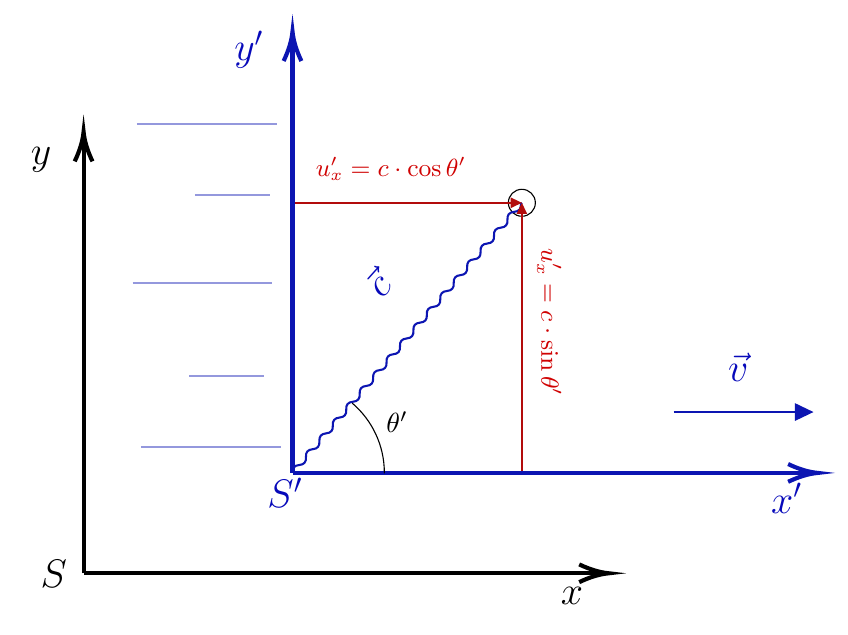
\begin{tikzpicture}[x=0.75pt,y=0.75pt,yscale=-1,xscale=1]
%uncomment if require: \path (0,408); %set diagram left start at 0, and has height of 408

%Straight Lines [id:da035704593072243496] 
\draw [line width=1.5]    (94.67,358.01) -- (94.67,148.34) ;
\draw [shift={(94.67,145.34)}, rotate = 90] [color={rgb, 255:red, 0; green, 0; blue, 0 }  ][line width=1.5]    (14.21,-4.28) .. controls (9.04,-1.82) and (4.3,-0.39) .. (0,0) .. controls (4.3,0.39) and (9.04,1.82) .. (14.21,4.28)   ;
%Straight Lines [id:da6185871938411547] 
\draw [line width=1.5]    (94.67,358.01) -- (344.67,358.01) ;
\draw [shift={(347.67,358.01)}, rotate = 180] [color={rgb, 255:red, 0; green, 0; blue, 0 }  ][line width=1.5]    (14.21,-4.28) .. controls (9.04,-1.82) and (4.3,-0.39) .. (0,0) .. controls (4.3,0.39) and (9.04,1.82) .. (14.21,4.28)   ;
%Straight Lines [id:da699063725695984] 
\draw [color={rgb, 255:red, 12; green, 21; blue, 178 }  ,draw opacity=1 ][line width=1.5]    (195.33,309.66) -- (195.33,99.99) ;
\draw [shift={(195.33,96.99)}, rotate = 90] [color={rgb, 255:red, 12; green, 21; blue, 178 }  ,draw opacity=1 ][line width=1.5]    (14.21,-4.28) .. controls (9.04,-1.82) and (4.3,-0.39) .. (0,0) .. controls (4.3,0.39) and (9.04,1.82) .. (14.21,4.28)   ;
%Straight Lines [id:da10168494105738768] 
\draw [color={rgb, 255:red, 12; green, 21; blue, 178 }  ,draw opacity=1 ][line width=1.5]    (195.33,309.66) -- (445.33,309.66) ;
\draw [shift={(448.33,309.66)}, rotate = 180] [color={rgb, 255:red, 12; green, 21; blue, 178 }  ,draw opacity=1 ][line width=1.5]    (14.21,-4.28) .. controls (9.04,-1.82) and (4.3,-0.39) .. (0,0) .. controls (4.3,0.39) and (9.04,1.82) .. (14.21,4.28)   ;
%Straight Lines [id:da19935241186224828] 
\draw [color={rgb, 255:red, 12; green, 21; blue, 178 }  ,draw opacity=1 ][line width=0.75]    (379,280.33) -- (443.33,280.33) ;
\draw [shift={(446.33,280.33)}, rotate = 180] [fill={rgb, 255:red, 12; green, 21; blue, 178 }  ,fill opacity=1 ][line width=0.08]  [draw opacity=0] (8.93,-4.29) -- (0,0) -- (8.93,4.29) -- cycle    ;
%Shape: Circle [id:dp5740094199155588] 
\draw   (299.33,179.51) .. controls (299.33,175.92) and (302.24,173.01) .. (305.83,173.01) .. controls (309.42,173.01) and (312.33,175.92) .. (312.33,179.51) .. controls (312.33,183.1) and (309.42,186.01) .. (305.83,186.01) .. controls (302.24,186.01) and (299.33,183.1) .. (299.33,179.51) -- cycle ;
%Straight Lines [id:da39046452059581926] 
\draw [color={rgb, 255:red, 12; green, 21; blue, 178 }  ,draw opacity=1 ][line width=0.75]    (195.33,309.66) .. controls (195.14,307.31) and (196.22,306.04) .. (198.57,305.85) .. controls (200.92,305.66) and (202,304.39) .. (201.81,302.04) .. controls (201.62,299.69) and (202.69,298.42) .. (205.04,298.23) .. controls (207.39,298.04) and (208.47,296.77) .. (208.28,294.42) .. controls (208.09,292.07) and (209.16,290.8) .. (211.51,290.6) .. controls (213.86,290.41) and (214.94,289.14) .. (214.75,286.79) .. controls (214.56,284.44) and (215.64,283.17) .. (217.99,282.98) .. controls (220.34,282.79) and (221.41,281.52) .. (221.22,279.17) .. controls (221.03,276.82) and (222.11,275.55) .. (224.46,275.36) .. controls (226.81,275.17) and (227.88,273.9) .. (227.69,271.55) .. controls (227.5,269.2) and (228.58,267.92) .. (230.93,267.73) .. controls (233.28,267.54) and (234.36,266.27) .. (234.17,263.92) .. controls (233.98,261.57) and (235.05,260.3) .. (237.4,260.11) .. controls (239.75,259.92) and (240.83,258.65) .. (240.64,256.3) .. controls (240.45,253.95) and (241.52,252.68) .. (243.87,252.49) .. controls (246.22,252.3) and (247.3,251.03) .. (247.11,248.68) .. controls (246.92,246.33) and (248,245.06) .. (250.35,244.87) .. controls (252.7,244.67) and (253.77,243.4) .. (253.58,241.05) .. controls (253.39,238.7) and (254.47,237.43) .. (256.82,237.24) .. controls (259.17,237.05) and (260.24,235.78) .. (260.05,233.43) .. controls (259.86,231.08) and (260.94,229.81) .. (263.29,229.62) .. controls (265.64,229.43) and (266.72,228.16) .. (266.53,225.81) .. controls (266.34,223.46) and (267.41,222.19) .. (269.76,222) .. controls (272.11,221.81) and (273.19,220.53) .. (273,218.18) .. controls (272.81,215.83) and (273.88,214.56) .. (276.23,214.37) .. controls (278.58,214.18) and (279.66,212.91) .. (279.47,210.56) .. controls (279.28,208.21) and (280.36,206.94) .. (282.71,206.75) .. controls (285.06,206.56) and (286.13,205.29) .. (285.94,202.94) .. controls (285.75,200.59) and (286.83,199.32) .. (289.18,199.13) .. controls (291.53,198.94) and (292.61,197.66) .. (292.42,195.31) .. controls (292.23,192.96) and (293.3,191.69) .. (295.65,191.5) .. controls (298,191.31) and (299.08,190.04) .. (298.89,187.69) .. controls (298.7,185.34) and (299.77,184.07) .. (302.12,183.88) .. controls (304.47,183.69) and (305.55,182.42) .. (305.36,180.07) -- (305.83,179.51) -- (305.83,179.51) ;
%Straight Lines [id:da2956236916778816] 
\draw [color={rgb, 255:red, 12; green, 21; blue, 178 }  ,draw opacity=0.44 ][line width=0.75]    (120.33,141.66) -- (187.67,141.66) ;
%Straight Lines [id:da06275454047861562] 
\draw [color={rgb, 255:red, 12; green, 21; blue, 178 }  ,draw opacity=0.44 ][line width=0.75]    (148.33,175.66) -- (184.33,175.66) ;
%Straight Lines [id:da6151819284038151] 
\draw [color={rgb, 255:red, 12; green, 21; blue, 178 }  ,draw opacity=0.44 ][line width=0.75]    (118.33,218.33) -- (185.67,218.33) ;
%Straight Lines [id:da4492087263895772] 
\draw [color={rgb, 255:red, 12; green, 21; blue, 178 }  ,draw opacity=0.44 ][line width=0.75]    (122.33,296.99) -- (189.67,296.99) ;
%Straight Lines [id:da6632850248594533] 
\draw [color={rgb, 255:red, 12; green, 21; blue, 178 }  ,draw opacity=0.44 ][line width=0.75]    (145.67,262.99) -- (181.67,262.99) ;
%Straight Lines [id:da3436387173601163] 
\draw [color={rgb, 255:red, 178; green, 12; blue, 12 }  ,draw opacity=1 ][line width=0.75]    (196.33,179.51) -- (302.83,179.51) ;
\draw [shift={(305.83,179.51)}, rotate = 180] [fill={rgb, 255:red, 178; green, 12; blue, 12 }  ,fill opacity=1 ][line width=0.08]  [draw opacity=0] (5.36,-2.57) -- (0,0) -- (5.36,2.57) -- cycle    ;
%Straight Lines [id:da6284992247502972] 
\draw [color={rgb, 255:red, 178; green, 12; blue, 12 }  ,draw opacity=1 ][line width=0.75]    (305.83,308.68) -- (305.83,182.51) ;
\draw [shift={(305.83,179.51)}, rotate = 90] [fill={rgb, 255:red, 178; green, 12; blue, 12 }  ,fill opacity=1 ][line width=0.08]  [draw opacity=0] (5.36,-2.57) -- (0,0) -- (5.36,2.57) -- cycle    ;
%Shape: Arc [id:dp25464527059767583] 
\draw  [draw opacity=0] (224.1,276.03) .. controls (233.58,284.15) and (239.58,296.2) .. (239.58,309.66) .. controls (239.58,309.74) and (239.58,309.82) .. (239.58,309.89) -- (195.33,309.66) -- cycle ; \draw   (224.1,276.03) .. controls (233.58,284.15) and (239.58,296.2) .. (239.58,309.66) .. controls (239.58,309.74) and (239.58,309.82) .. (239.58,309.89) ;  

% Text Node
\draw (68,151.41) node [anchor=north west][inner sep=0.75pt]  [font=\Large]  {$y$};
% Text Node
\draw (323.33,363.41) node [anchor=north west][inner sep=0.75pt]  [font=\Large]  {$x$};
% Text Node
\draw (166,95.41) node [anchor=north west][inner sep=0.75pt]  [font=\Large,color={rgb, 255:red, 7; green, 9; blue, 186 }  ,opacity=1 ]  {$y'$};
% Text Node
\draw (424.67,313.41) node [anchor=north west][inner sep=0.75pt]  [font=\Large,color={rgb, 255:red, 7; green, 9; blue, 186 }  ,opacity=1 ]  {$x'$};
% Text Node
\draw (72.67,350.41) node [anchor=north west][inner sep=0.75pt]  [font=\Large]  {$S$};
% Text Node
\draw (182,310.74) node [anchor=north west][inner sep=0.75pt]  [font=\Large,color={rgb, 255:red, 7; green, 9; blue, 186 }  ,opacity=1 ]  {$S'$};
% Text Node
\draw (404,250.74) node [anchor=north west][inner sep=0.75pt]  [font=\Large,color={rgb, 255:red, 7; green, 9; blue, 186 }  ,opacity=1 ]  {$\vec{v}$};
% Text Node
\draw (226.87,217.15) node [anchor=north west][inner sep=0.75pt]  [font=\Large,color={rgb, 255:red, 7; green, 9; blue, 186 }  ,opacity=1 ,rotate=-311.86]  {$\vec{c}$};
% Text Node
\draw (205.33,156.08) node [anchor=north west][inner sep=0.75pt]  [font=\small,color={rgb, 255:red, 208; green, 2; blue, 2 }  ,opacity=1 ]  {$u_{x} '=c\cdot \cos \theta '$};
% Text Node
\draw (326.1,200.51) node [anchor=north west][inner sep=0.75pt]  [font=\small,color={rgb, 255:red, 208; green, 2; blue, 2 }  ,opacity=1 ,rotate=-90]  {$u_{x} '=c\cdot \sin \theta '$};
% Text Node
\draw (239.33,278.74) node [anchor=north west][inner sep=0.75pt]    {$\theta '$};


\end{tikzpicture}
    \end{figure}

	
Notice that, in the $S'$ frame, the light has the following velocity components: $u_y' = c \sin{(\theta')}$ and $u_x' = c \cos{(\theta')}$. Applying the Lorentz velocity transformations:

$$dx' = \gamma (dx - v dt)$$
$$dy' = dy$$
$$dt' = \gamma \left( dt - \frac{v dx}{c^2} \right)$$

For the horizontal component:

$$u_x' = \frac{dx'}{dt'} = \frac{\gamma (dx - v dt)}{\gamma \left( dt - \frac{v dx}{c^2} \right)} = \frac{dx - v dt}{dt - \frac{v dx}{c^2}}$$

For $S$, the velocity component is $u_x = \frac{dx}{dt}$:

$$u_x' = \frac{u_x - v}{1 - \frac{v u_x}{c^2}}$$

Solving for $u_x$:

$$u_x = \frac{v + u_x'}{1 + \frac{v u_x'}{c^2}}$$

Since $u_x = c \cdot \cos{(\theta)}$ and $u_x' = c \cdot \cos{(\theta')}$, and recalling that $v = \beta c$:

$$\cos{(\theta)} = \frac{\beta + \cos{(\theta')}}{1 + \beta \cos{(\theta')}}$$

\textbf{Note:} This relation alone is sufficient to relate the angles, but working with the sine will be very useful.

For $u_y'$:

$$u_y' = \frac{dy'}{dt'} = \frac{dy}{\gamma \left( dt - \frac{v dx}{c^2} \right)} = \frac{u_y}{\gamma \left( 1 - \frac{v u_x}{c^2} \right)}$$

Since $u_x = c \cos{(\theta)}$, $u_y = c \sin{(\theta)}$, and $u_y' = c \sin{(\theta')}$:

$$\sin{(\theta)} = \frac{\sin{(\theta')}}{\gamma \left( 1 + \beta \cos{(\theta')} \right)}$$

\ut{B.3} It is sufficient to differentiate the obtained expressions:

$$d\sin{(\theta)} = d\frac{\sin{(\theta')}}{\gamma \left( 1 + \beta \cos{(\theta')} \right)}$$

$$\cos{(\theta)} d\theta = \frac{1}{\gamma} \frac{\beta + \cos{(\theta')}}{(1 + \beta \cos{(\theta')})^2} d\theta'$$

Using the cosine relations used previously and rearranging:

$$\frac{d\theta}{\gamma (1 - \beta \cos{(\theta)})} = d\theta'$$

\begin{doublespace}

\begin{large}
\textbf{Part C: Redshift and Blueshift}
\end{large}

\end{doublespace}

\ut{C.1} Recall the dot product of two vectors: $\vec{v} \cdot \vec{u} = v_x u_x + v_y u_y$, thus:

$$\vec{k} \cdot \vec{r} = k_y y + k_x x$$

We can separate the components of $\vec{k}$ based on the propagation angle:

$$\vec{k} \cdot \vec{r} = k \sin{(\theta)} y + k \cos{(\theta)} x$$

Substituting the Lorentz transformations:

$$\vec{k} \cdot \vec{r} - \omega t = k \sin{(\theta)} y' + k \cos{(\theta)} \gamma (x' + v t') - \omega \gamma \left( t' + \frac{v x'}{c^2} \right)$$

\ut{C.2} For $S'$:

$$\phi' = \vec{k'} \cdot \vec{r'} - \omega' t'$$

Notice that both equations (the previous item and this one) describe the same wave function in the $S'$ frame, so we can associate the terms. All terms accompanying $t'$ correspond to the frequency $\omega'$:

$$k \cos{(\theta)} \gamma (v t') - \omega \gamma (t') = -\omega' t'$$

Since $k = \frac{2 \pi}{\lambda} = \frac{2 \pi f}{c}$ and $\omega = 2 \pi f$:

$$\left( \frac{v}{c} \cos{(\theta)} - 1 \right) 2 \pi \gamma f = -2 \pi f'$$

Finally:

$$f = \frac{f'}{\gamma (1 - \beta \cos{(\theta)})}$$

\begin{doublespace}

\begin{large}
\textbf{Part D: The Grand Unification}
\end{large}

\end{doublespace}

\ut{D.1} Considering the angular interval, the energy $dE$ is the product of the number of photons passing through the area section and the energy of each photon. Therefore:

$$\frac{dE}{dt} = \frac{n E}{dt}$$

And for $S'$, the number of photons passing through the section is the same (even with angular changes, the number of photons remains unchanged):

$$\frac{dE'}{dt'} = \frac{n E'}{dt'}$$

Recalling that $E = hf = hf' \frac{1}{\gamma (1 - \beta \cos{(\theta)})} = \frac{E'}{\gamma (1 - \beta \cos{(\theta)})}$ and that $dt = \gamma dt'$ (time dilation):

$$\frac{dE}{dt} = \frac{1}{(1 - \beta \cos{(\theta)}) \gamma^2} \frac{dE'}{dt'}$$

\ut{D.2} From this, we have:

$$dL(\theta) = \frac{1}{(1 - \beta \cos{(\theta)}) \gamma^2} dL'$$

$$dL(\theta) = \frac{1}{(1 - \beta \cos{(\theta)}) \gamma^2} \frac{L}{2} \sin{(\theta')} d\theta'$$

Substituting the relations for $\sin{(\theta')}$ and $d\theta'$ found in item B.3:

$$dL(\theta) = \frac{L}{2 \gamma^4} \frac{\sin{(\theta)} d\theta}{(1 - \beta \cos{(\theta)})^3}$$

\ut{D.3} Integrating the luminosity from $0$ to $L_t$ and the angle from $\pi$ to $0$:

$$\int_0^{L_t} dL(\theta) = \int_{\pi}^0 \frac{L}{2 \gamma^4} \frac{\sin{(\theta)} d\theta}{(1 - \beta \cos{(\theta)})^3}$$

Since $\sin{(\theta)} d\theta = d\cos{(\theta)}$ and substituting $\cos{(\theta)} = u$:

$$L_t = \frac{L}{2 \gamma^4} \int_{\pi}^0 \frac{d\cos{(\theta)}}{(1 - \beta \cos{(\theta)})^3} = \frac{L}{2 \gamma^4} \int_{-1}^{1} \frac{du}{(1 - \beta u)^3}$$

Substituting $z = 1 - \beta u$, so $dz = -\beta du$:

$$L_t = -\frac{L}{2 \beta \gamma^4} \int_{1+\beta}^{1-\beta} \frac{dz}{z^3}$$

Finally:

$$L_t = \frac{L}{4 \beta \gamma^4} \left( \frac{1}{(1 - \beta)^2} - \frac{1}{(1 + \beta)^2} \right)$$

Notice that:

$$\left( \frac{1}{(1 - \beta)^2} - \frac{1}{(1 + \beta)^2} \right) = \frac{1 + 2\beta + \beta^2 - 1 + 2\beta - \beta^2}{(1 - \beta^2)^2} = 4 \beta \gamma^4$$

Therefore: $L_t = L$

\textbf{EXTRA:} Imagine a star whose energy is given solely by its rest mass. Its energy in $S'$ is $E' = m_0 c^2$, while in $S$ it is $E = \gamma m_0 c^2$. Note that the rest mass is the same in both frames (by definition). Considering luminosity as the rate of energy change over time:

$$L = \frac{dE}{dt} = \frac{\gamma c^2 dm_0}{dt}$$

Substituting $dt = \gamma dt'$:

$$L = \frac{dE}{dt} = \frac{\gamma c^2 dm_0}{\gamma dt'} = L'$$

Which confirms the result obtained!
	
	\clearpage
    
    
    \fi
\end{document}
